\chapter{Mencampur dan Melarutkan}\label{ch:g2:mixing-and-dissolving}

Sebutir gula batu jatuh ke dalam secangkir teh panas. Sendok mengaduk,
gula batu itu hancur, dan sesaat kemudian tidak ada lagi yang terlihat:
tehnya tampak persis seperti tadi. Namun sekarang tehnya terasa manis.
Gula itu tidak pergi --- ia bersembunyi di dalam teh. Bab ini membahas
cara menyatukan berbagai benda, dan benda-benda yang seolah-olah lenyap
ketika kita melakukannya.

\begin{omfigure}
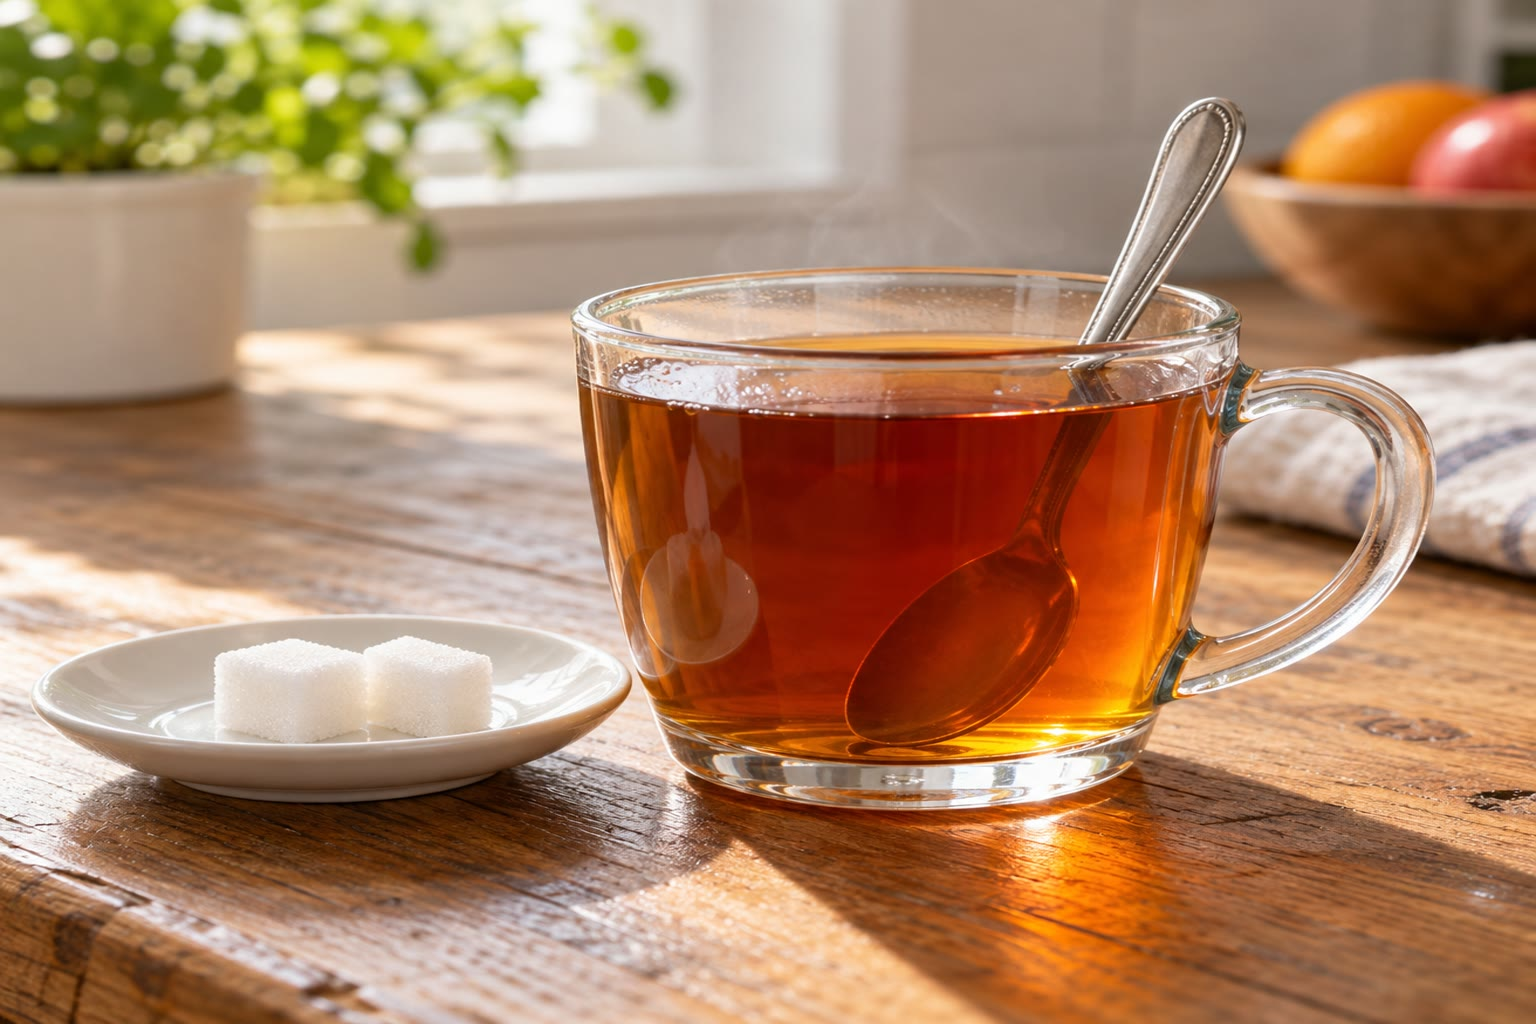
\includegraphics[width=0.55\linewidth]{images/book1/ai/g2-tea-sugar.jpg}

{\small Secangkir teh dan dua gula batu. Setelah diaduk, gula itu hilang
dari pandangan, tetapi tidak hilang dari rasanya.}
\end{omfigure}

\section{Mencampur berbagai benda}

\begin{definition}[Mencampur]\label{def:g2:mixing-and-dissolving:mix}
Yang disebut \emph{mencampur}\index{mencampur} adalah menyatukan
benda-benda yang berbeda, dan sering kali mengaduknya. Yang kita peroleh
adalah campuran benda-benda itu.
\end{definition}

\begin{example}[Semangkuk muesli]\label{ex:g2:mixing-and-dissolving:muesli}
Gandum, kismis, kacang, dan biji-bijian dituang ke dalam satu mangkuk:
itulah sebuah campuran. Kalau diperhatikan baik-baik, setiap bahannya
masih terlihat dan masih dapat dipungut lagi dengan jari --- kismis
tetap kismis, kacang tetap kacang.
\end{example}

\begin{example}[Sirop dalam air]\label{ex:g2:mixing-and-dissolving:syrup}
Dua cairan pun dapat \omterm{def:g2:mixing-and-dissolving:mix}{dicampur}. Sirop merah yang dituang ke segelas air
tenggelam membentuk gulungan warna; setelah diaduk, seluruh isi gelas
berwarna merah muda yang rata. Sirop dan air tidak dapat lagi dibedakan
dengan mata.
\end{example}

\begin{omfigure}
\begin{minipage}[t]{0.48\linewidth}\centering
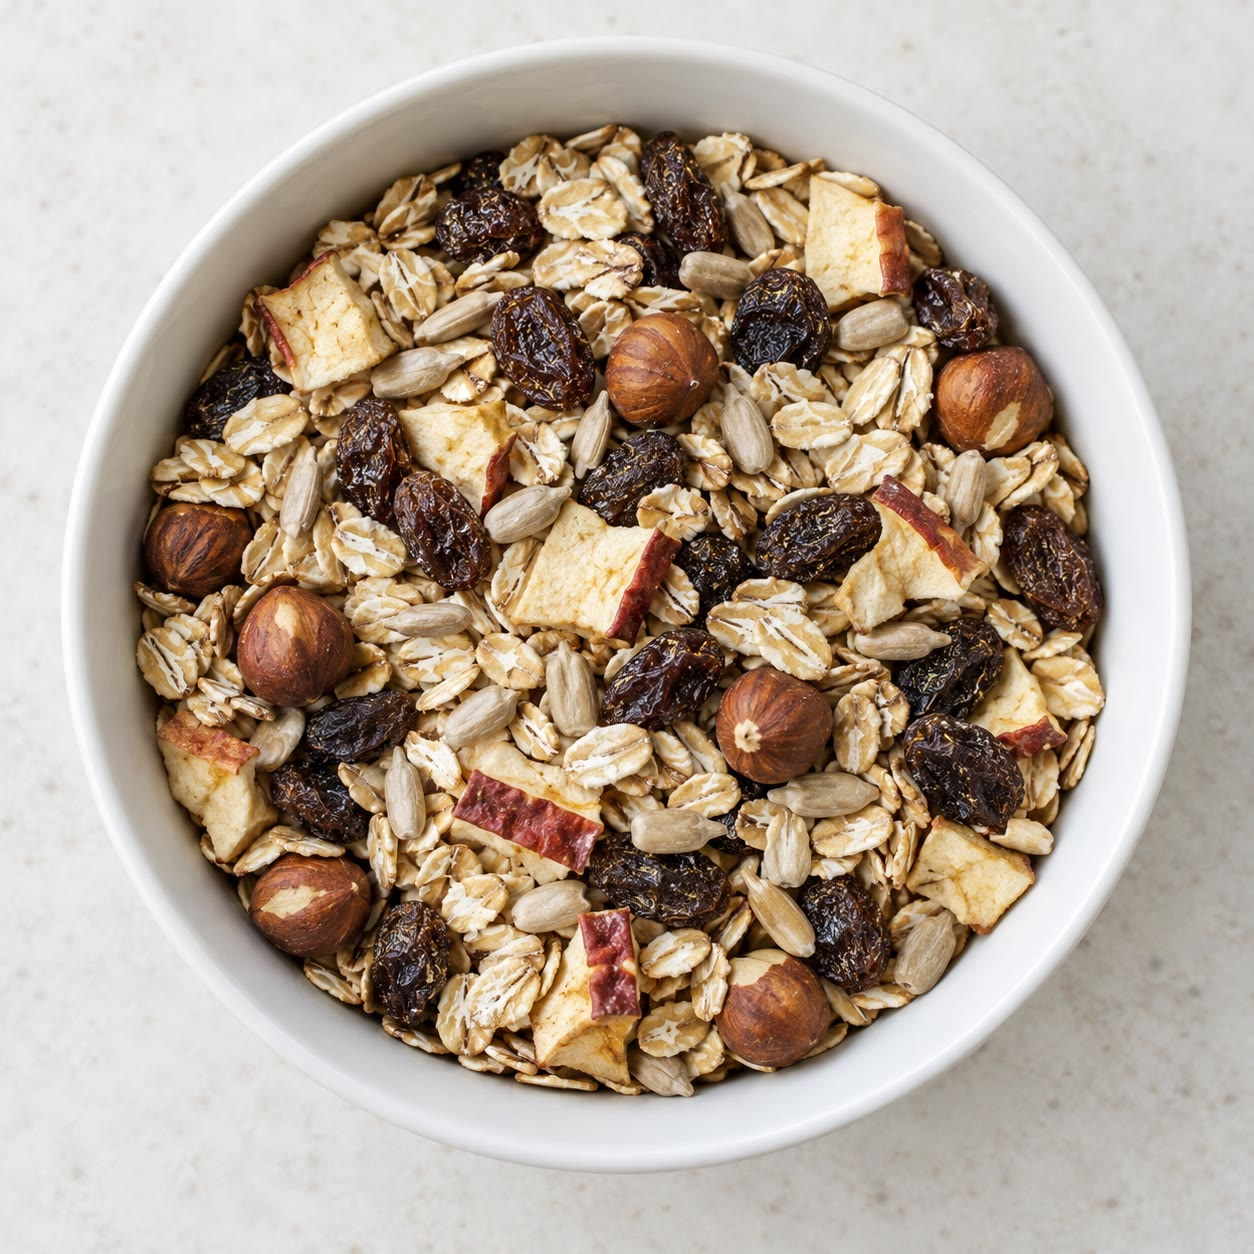
\includegraphics[width=\linewidth,height=4.6cm,keepaspectratio]{images/book1/ai/g2-muesli.jpg}

{\small Muesli: campuran yang setiap bagiannya masih terlihat.}
\end{minipage}\hfill
\begin{minipage}[t]{0.48\linewidth}\centering
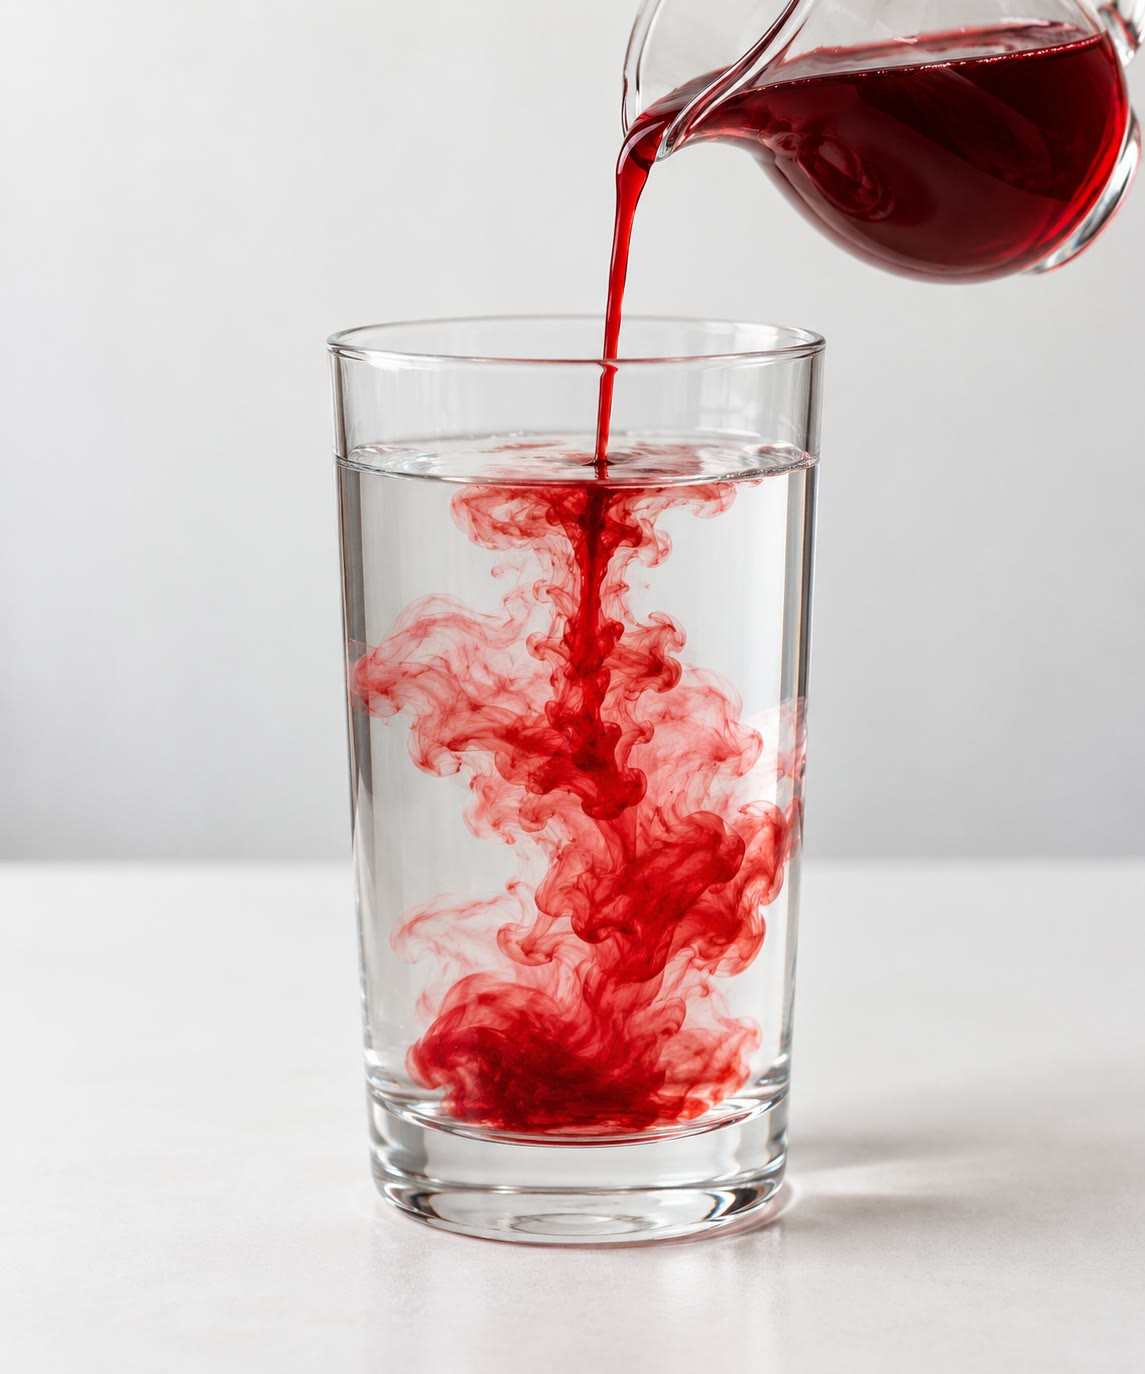
\includegraphics[width=\linewidth,height=4.6cm,keepaspectratio]{images/book1/ai/g2-syrup-in-water.jpg}

{\small Sirop dituang ke dalam air: dua cairan bercampur.}
\end{minipage}
\end{omfigure}

\begin{remark}[Mencampur tidak merusak apa pun]\label{rem:g2:mixing-and-dissolving:nothing-lost}
Ketika benda-benda \omterm{def:g2:mixing-and-dissolving:mix}{dicampur}, tidak ada yang hilang dan tidak ada yang
baru terbentuk. Gandum, kismis, dan kacang semuanya masih ada di dalam
mangkuk. Sebuah bab berikutnya menunjukkan cara memisahkan lagi sebuah
campuran.
\end{remark}

\section{Benda yang larut}

\begin{definition}[Melarut dan larutan]\label{def:g2:mixing-and-dissolving:dissolve}
Suatu padatan \emph{larut}\index{larut} dalam air jika, setelah
\omterm{def:g2:mixing-and-dissolving:mix}{dicampurkan} ke dalam air dan diaduk, padatan itu hilang dari pandangan
dan membiarkan cairannya \emph{jernih}, artinya tembus pandang. Gula dan
garam larut dalam air. Cairan jernih yang kita peroleh disebut
\emph{larutan}\index{larutan}: air gula adalah larutan gula, air
asin adalah larutan garam.
\end{definition}

\begin{example}[Sebutir gula batu dalam segelas air]\label{ex:g2:mixing-and-dissolving:cube}
Sebutir gula batu diletakkan di dasar segelas air yang tenang.
Sudut-sudutnya melunak, ukurannya mengecil, dan alur-alur bergelombang
naik darinya menembus air. Kalau kita mengaduk, gula itu habis dalam
satu menit. Kalau tidak diaduk, gula itu tetap hilang, hanya jauh lebih
lambat.
\end{example}

\begin{remark}[Jernih tidak sama dengan tak berwarna]\label{rem:g2:mixing-and-dissolving:clear}
Teh berwarna cokelat dan air sirop berwarna merah muda, tetapi kita
dapat melihat menembus keduanya: keduanya jernih. \omterm{def:g2:mixing-and-dissolving:dissolve}{Larutan} boleh
berwarna. Yang tidak pernah ada pada \omterm{def:g2:mixing-and-dissolving:dissolve}{larutan} adalah butiran yang
melayang di dalamnya atau lapisan di dasarnya.
\end{remark}

\begin{method}[Larutkah?]\label{met:g2:mixing-and-dissolving:test}
Untuk mengetahui apakah suatu padatan \omterm{def:g2:mixing-and-dissolving:dissolve}{larut} dalam air:
\begin{enumerate}
  \item masukkan sedikit padatan itu ke dalam segelas air;
  \item aduklah, lalu tunggu beberapa menit;
  \item lihatlah menembus gelas:
    \begin{itemize}
      \item jernih, dan tidak ada apa-apa di dasar: padatan itu \omterm{def:g2:mixing-and-dissolving:dissolve}{larut};
      \item keruh, atau ada lapisan di dasar: padatan itu tidak \omterm{def:g2:mixing-and-dissolving:dissolve}{larut}.
    \end{itemize}
\end{enumerate}
\end{method}

\section{Benda yang tidak larut}

\begin{proposition}[Pasir dan kapur tulis tidak larut]\label{prop:g2:mixing-and-dissolving:not}
Banyak padatan tidak \omterm{def:g2:mixing-and-dissolving:dissolve}{larut} dalam air: pasir, kapur tulis, tanah,
kerikil, tepung. Kalau diaduk ke dalam air, padatan itu membuat air
keruh; kalau dibiarkan, padatan itu turun dan mengendap di dasar, dan
air di atasnya kembali lebih jernih. Selama apa pun kita mengaduk,
padatan itu tidak pernah hilang.
\end{proposition}

\begin{example}[Sestoples air berlumpur]\label{ex:g2:mixing-and-dissolving:mud}
Tanah kebun yang dikocok dalam stoples berisi air membuat airnya cokelat
dan keruh. Sejam kemudian, tanah dan kerikil kecil berada dalam lapisan
gelap di dasar, beberapa daun kering terapung di atas, dan air di
antaranya hanya sedikit keruh. Tanah itu tidak \omterm{def:g2:mixing-and-dissolving:dissolve}{larut}.
\end{example}

\begin{omfigure}
\begin{minipage}[t]{0.48\linewidth}\centering
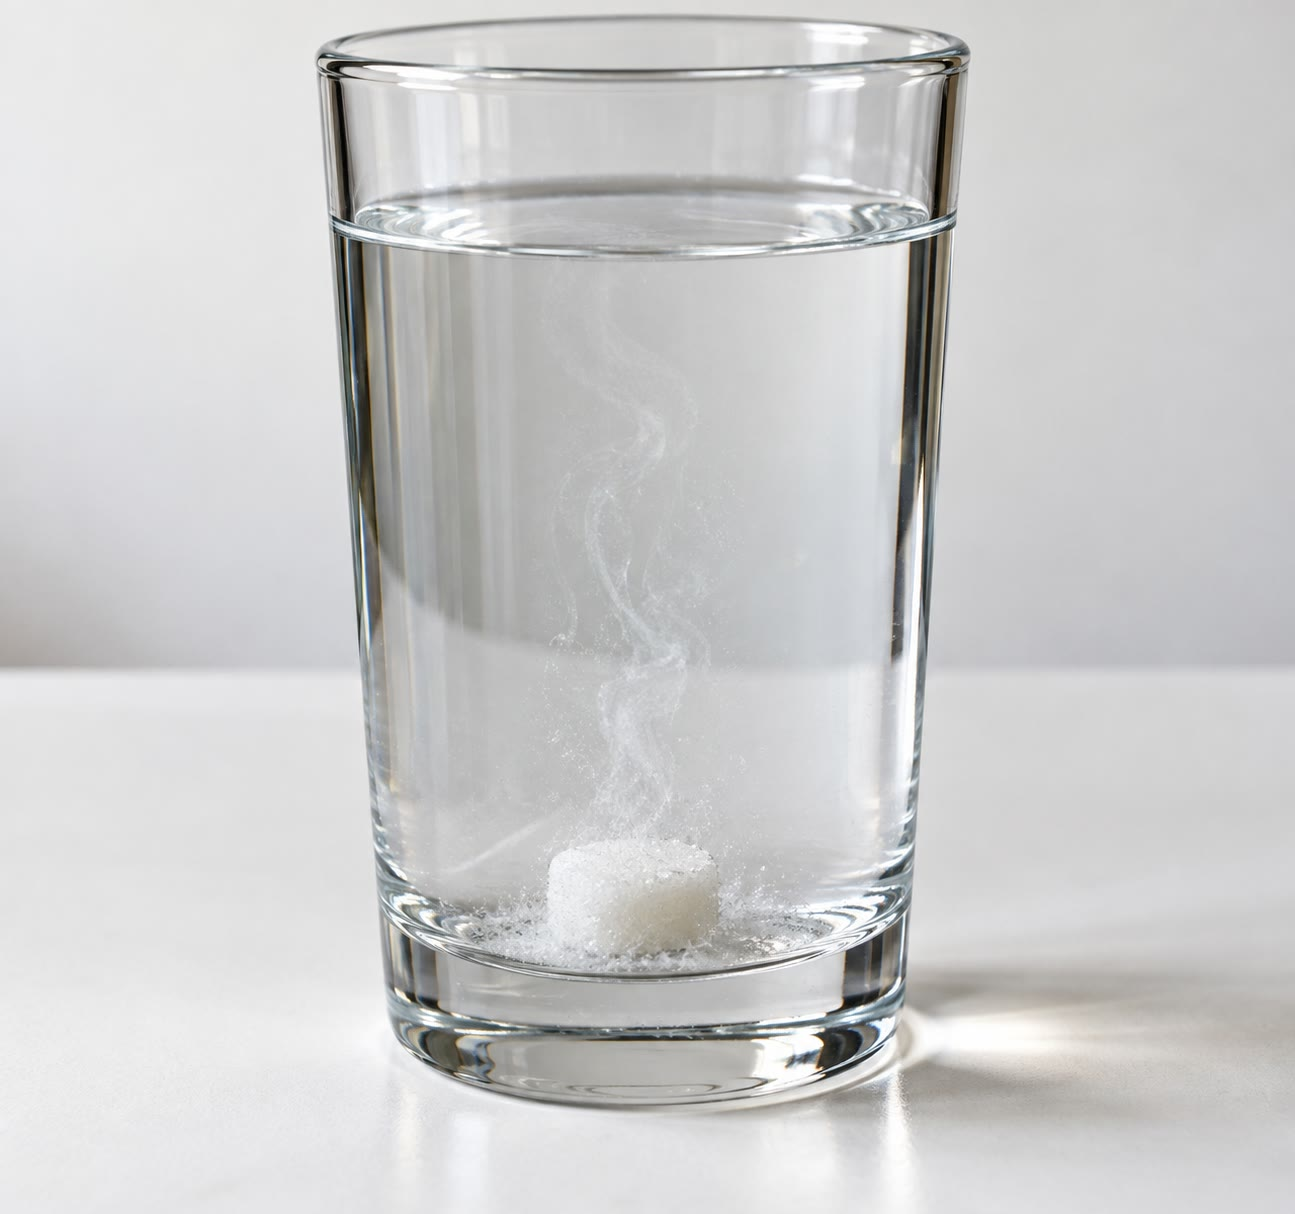
\includegraphics[width=\linewidth,height=4.6cm,keepaspectratio]{images/book1/ai/g2-sugar-cube-dissolving.jpg}

{\small Gula yang sedang \omterm{def:g2:mixing-and-dissolving:dissolve}{larut}: alur-alur naik dari gula batu.}
\end{minipage}\hfill
\begin{minipage}[t]{0.48\linewidth}\centering
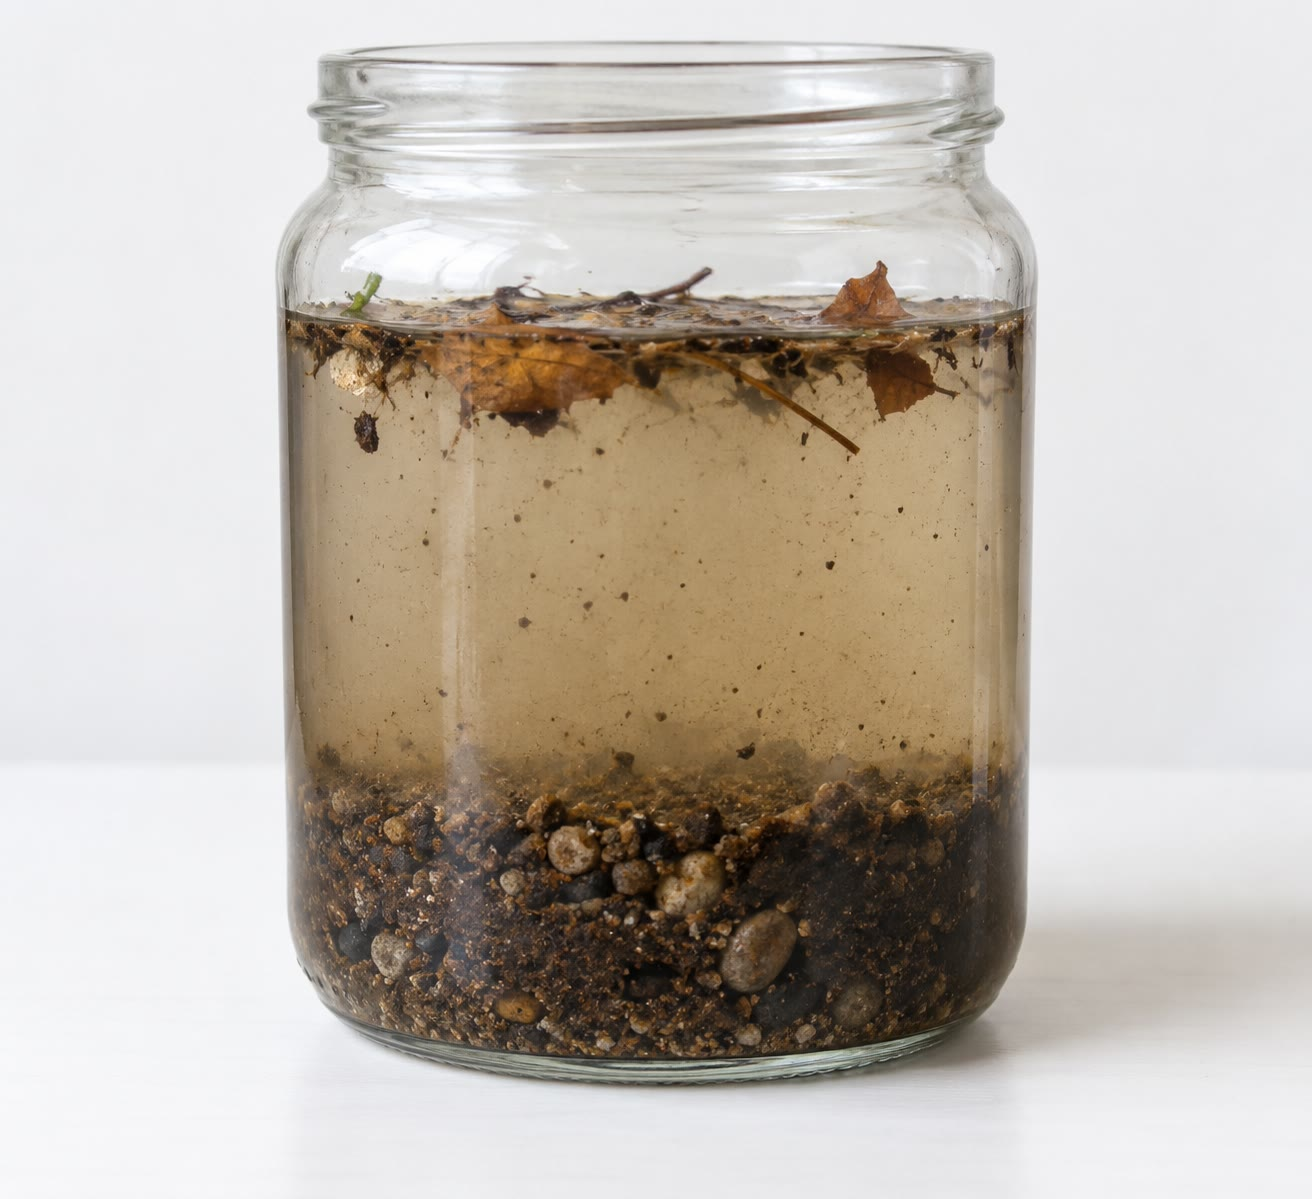
\includegraphics[width=\linewidth,height=4.6cm,keepaspectratio]{images/book1/ai/g2-muddy-jar.jpg}

{\small Tanah tidak \omterm{def:g2:mixing-and-dissolving:dissolve}{larut}: tanah itu mengendap di dasar.}
\end{minipage}
\end{omfigure}

\begin{omfigure}
\begin{tikzpicture}[font=\small, scale=1.35]
  \pic[transform shape] at (0,0) {beaker={0.7}{omWater!70}};
  \fill[brown!55] (4.2,0) rectangle (5.8,0.22);
  \pic[transform shape] at (5,0) {beaker={0.7}{brown!12}};
  \fill[brown!55] (4.2,0) rectangle (5.8,0.22);
  \draw[omGlass, line width=0.7pt] (4.2,0.22) -- (4.2,0) -- (5.8,0) -- (5.8,0.22);
  \foreach \x/\y in {4.4/0.32,4.75/0.45,5.1/0.3,5.5/0.5,4.6/0.7,5.3/0.8,4.9/1.0}
    \fill[brown!60] (\x,\y) circle (0.025);
  \node[align=center, anchor=north] at (0,-0.15)
    {\textbf{gula} dalam air, diaduk:\\ jernih, dasar kosong};
  \node[align=center, anchor=north] at (5,-0.15)
    {\textbf{pasir} dalam air, diaduk:\\ keruh, ada lapisan di dasar};
  \draw[<-, omProp, thick] (6.0,0.11) -- (7.0,0.11)
    node[right, text=black] {pasirnya};
\end{tikzpicture}

{\small Uji pada \cref{met:g2:mixing-and-dissolving:test}: gula \omterm{def:g2:mixing-and-dissolving:dissolve}{larut},
pasir tidak.}
\end{omfigure}

\section{Yang larut masih ada di sana}

\begin{proposition}[Padatan yang larut masih ada di dalam air]\label{prop:g2:mixing-and-dissolving:still-there}
Ketika suatu padatan \omterm{def:g2:mixing-and-dissolving:dissolve}{larut}, padatan itu tidak lenyap: ia tersebar ke
seluruh air, dalam bagian-bagian yang jauh terlalu kecil untuk dilihat.
Dua petunjuk menunjukkan bahwa padatan itu masih ada:
\begin{itemize}
  \item teh manis terasa manis, dan air laut terasa asin;
  \item ketika airnya mengering, padatan itu tertinggal.
\end{itemize}
\end{proposition}

\begin{remark}[Tidak ada yang mencicipi di laboratorium]\label{rem:g2:mixing-and-dissolving:no-tasting}
Kita tahu bahwa teh itu manis karena teh adalah minuman. Di
laboratorium, tidak seorang pun pernah mencicipi apa pun, bahkan cairan
yang tampak seperti air: petunjuk kedua, yaitu membiarkan airnya
mengering, adalah petunjuk yang dipakai para ahli kimia.
\end{remark}

\begin{example}[Garam dari laut]\label{ex:g2:mixing-and-dissolving:salt-pans}
Di beberapa pantai yang cerah, air laut dialirkan ke kolam-kolam yang
lebar dan dangkal. Hari demi hari, matahari mengeringkan airnya. Yang
tersisa di dasar adalah garam putih, yang dikumpulkan menjadi
tumpukan: itulah garam yang tadinya \omterm{def:g2:mixing-and-dissolving:dissolve}{larut} di laut. Garam di meja makan
sering berasal dari kolam seperti itu.
\end{example}

\begin{omfigure}
\begin{tikzpicture}[font=\small, scale=1.25]
  % day 1: a saucer of salty water
  \fill[omWater!80] (0,0.18) ellipse (1.25 and 0.22);
  \draw[omGlass, line width=0.7pt] (-1.5,0.3) .. controls (-1.2,-0.15) and (1.2,-0.15) .. (1.5,0.3);
  \draw[omGlass, line width=0.5pt] (0,0.3) ellipse (1.5 and 0.28);
  \node[align=center, anchor=north] at (0,-0.35) {sepiring kecil\\ air asin};
  % the sun
  \fill[ocYellow] (3.4,1.45) circle (0.28);
  \foreach \a in {0,45,...,315}
    \draw[ocYellow!90!orange, thick] ($(3.4,1.45)+(\a:0.36)$) -- ($(3.4,1.45)+(\a:0.52)$);
  \draw[->, thick, omProp] (2.0,0.3) -- (4.8,0.3)
    node[midway, below, text=black, align=center] {beberapa hari\\ cerah kemudian};
  % later: a white crust
  \begin{scope}[xshift=6.3cm]
    \draw[omGlass, line width=0.7pt] (-1.5,0.3) .. controls (-1.2,-0.15) and (1.2,-0.15) .. (1.5,0.3);
    \draw[omGlass, line width=0.5pt] (0,0.3) ellipse (1.5 and 0.28);
    \foreach \x/\y in {-0.9/0.12,-0.6/0.2,-0.3/0.08,0/0.18,0.3/0.1,0.6/0.2,0.9/0.12,
                       -0.45/0.28,0.15/0.27,0.75/0.3,-0.75/0.31}
      \fill[white, draw=black!45, line width=0.2pt] (\x,\y) rectangle ++(0.11,0.07);
    \node[align=center, anchor=north] at (0,-0.35) {airnya habis:\\ garam putih};
  \end{scope}
\end{tikzpicture}

{\small Airnya mengering; garam yang tadinya \omterm{def:g2:mixing-and-dissolving:dissolve}{larut} di dalamnya
tertinggal.}
\end{omfigure}

\begin{omfigure}
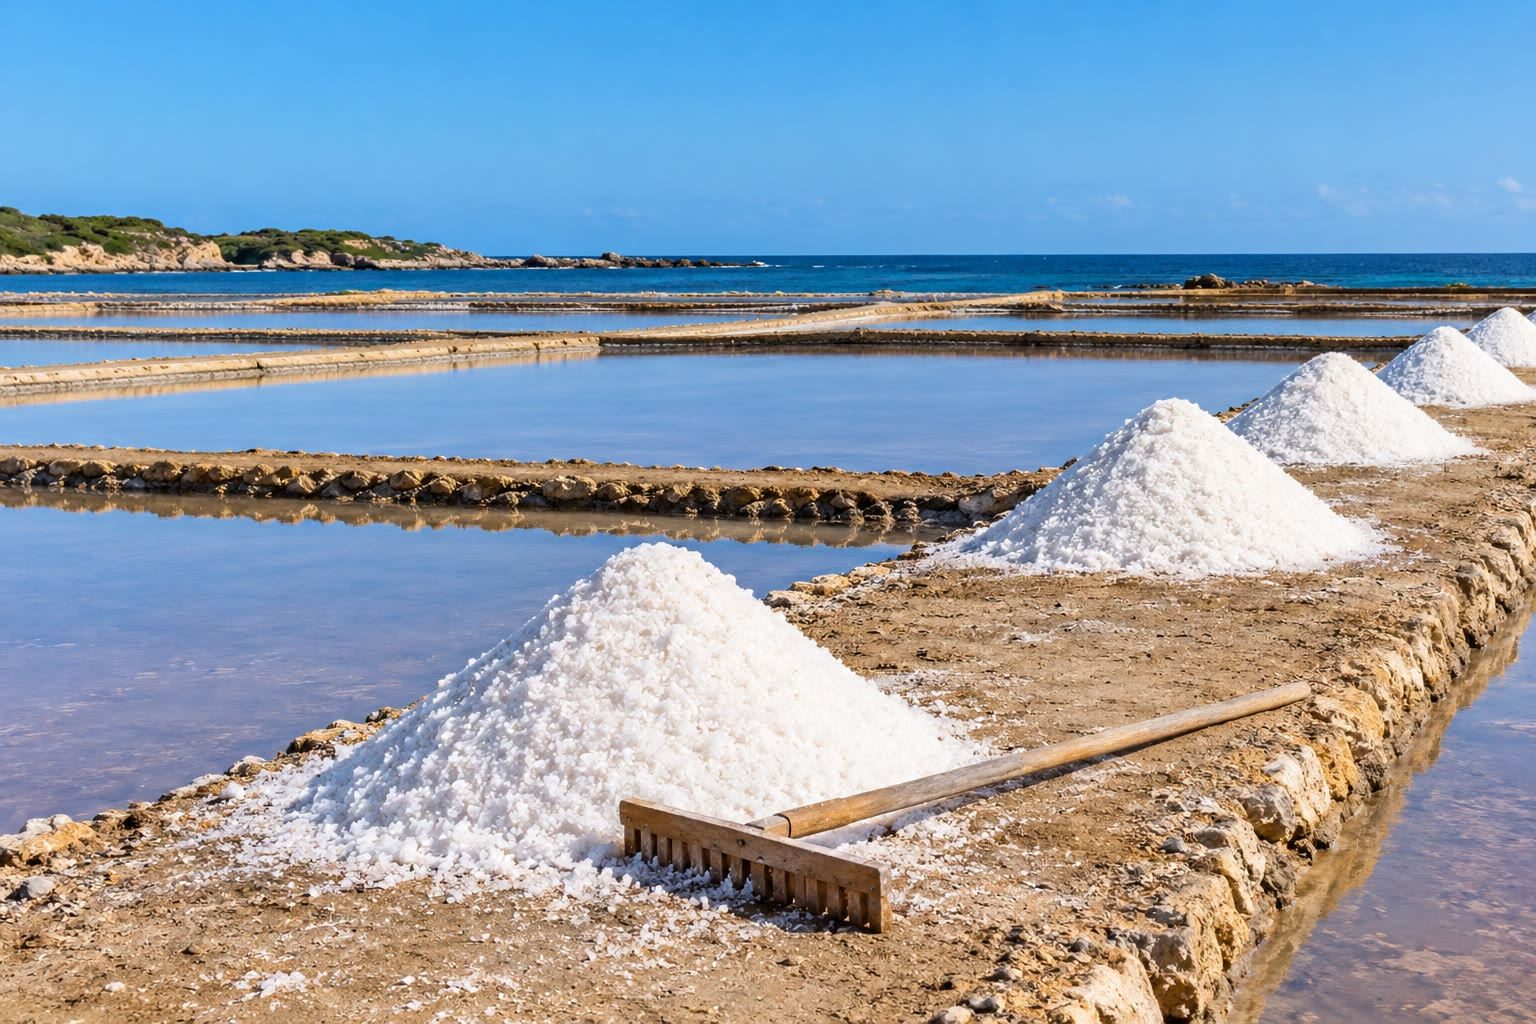
\includegraphics[width=0.62\linewidth]{images/book1/ai/g2-salt-pans.jpg}

{\small Tambak garam di tepi laut: matahari mengeringkan airnya, garam
tertinggal dalam tumpukan putih.}
\end{omfigure}

\begin{remark}[Melarut bukan mencair]\label{rem:g2:mixing-and-dissolving:not-melting}
Orang sering berkata bahwa gula ``mencair'' di dalam teh. Itu keliru:
mencair adalah yang terjadi pada es batu di bawah matahari, berubah
menjadi cairan dengan sendirinya, tanpa memerlukan air. Gula di dalam
teh memerlukan air, dan gula itu masih ada di dalamnya, tersebar. Kata
yang tepat adalah \emph{\omterm{def:g2:mixing-and-dissolving:dissolve}{larut}}.
\end{remark}

\section{Latihan}

\begin{exercise}[$\star$]\label{exo:g2:mixing-and-dissolving:1}
Manakah di antara padatan berikut yang \omterm{def:g2:mixing-and-dissolving:dissolve}{larut} dalam air, dan mana yang
tidak? Gula, pasir, garam, kapur tulis, kerikil.
\end{exercise}

\begin{exercise}[$\star$]\label{exo:g2:mixing-and-dissolving:2}
Apa itu \omterm{def:g2:mixing-and-dissolving:dissolve}{larutan}? Berikan dua contoh dari bab ini.
\end{exercise}

\begin{exercise}[$\star$]\label{exo:g2:mixing-and-dissolving:3}
Apakah semangkuk muesli itu campuran? Masihkah kamu dapat melihat
setiap bagiannya?
\end{exercise}

\begin{exercise}[$\star$]\label{exo:g2:mixing-and-dissolving:4}
Sejumlah serbuk putih diaduk ke dalam segelas air. Beberapa menit
kemudian, airnya keruh dan terbentuk lapisan putih di dasar. Apakah
serbuk itu \omterm{def:g2:mixing-and-dissolving:dissolve}{larut}? Jelaskan dengan
\cref{met:g2:mixing-and-dissolving:test}.
\end{exercise}

\begin{exercise}[$\star$]\label{exo:g2:mixing-and-dissolving:5}
Segelas air sirop berwarna merah muda. Apakah air itu jernih? Apakah
tak berwarna? Apakah air itu \omterm{def:g2:mixing-and-dissolving:dissolve}{larutan}?
\end{exercise}

\begin{exercise}[$\star$]\label{exo:g2:mixing-and-dissolving:6}
Setelah diaduk, tidak ada gula yang terlihat dalam secangkir teh.
Sebutkan petunjuk yang menunjukkan bahwa gula itu masih ada.
\end{exercise}

\begin{exercise}[$\star$]\label{exo:g2:mixing-and-dissolving:7}
Di tambak garam, apa yang diambil oleh matahari, dan apa yang
tertinggal?
\end{exercise}

\begin{exercise}[$\star$]\label{exo:g2:mixing-and-dissolving:8}
Tom berkata: ``Gulanya mencair di tehku.'' Kata apa yang seharusnya ia
pakai, dan mengapa?
\end{exercise}

\begin{exercise}[$\star\star$]\label{exo:g2:mixing-and-dissolving:9}
Lihatlah gambar dengan dua gelas kimia. Tanpa membaca tulisan di
bawahnya, bagaimana kamu dapat mengetahui gelas mana yang berisi pasir?
\end{exercise}

\begin{exercise}[$\star\star$]\label{exo:g2:mixing-and-dissolving:10}
Setetes air keran mengering di atas piring hitam dan meninggalkan
cincin putih kecil. Apa yang ditunjukkannya tentang air keran?
\end{exercise}

\begin{exercise}[$\star\star$]\label{exo:g2:mixing-and-dissolving:11}
Di laboratorium, seorang guru mempunyai dua gelas berisi cairan jernih
tak berwarna: yang satu berisi air murni, yang lain air asin. Tidak
seorang pun boleh mencicipinya. Bagaimana guru itu dapat mengetahui
mana yang mana?
\end{exercise}
